% $Header: /cvsroot/latex-beamer/latex-beamer/solutions/generic-talks/generic-ornate-15min-45min.en.tex,v 1.5 2007/01/28 20:48:23 tantau Exp $

\documentclass{beamer}

\usepackage{caption}
\captionsetup{labelformat=empty,labelsep=none,font=scriptsize}
\setlength{\abovecaptionskip}{0pt}

\usepackage{color}
%% These definitions are based on darkred at
%% http://www.december.com/html/spec/colorcmyk.html
\definecolor{darkred}{cmyk}{0, 1, 1, 0.45}
\newcommand{\jul}{\textcolor{darkred}}
\newcommand{\jan}{\textcolor{blue}}

% This file is a solution template for:

% - Giving a talk on some subject.
% - The talk is between 15min and 45min long.
% - Style is ornate.



% Copyright 2004 by Till Tantau <tantau@users.sourceforge.net>.
%
% In principle, this file can be redistributed and/or modified under
% the terms of the GNU Public License, version 2.
%
% However, this file is supposed to be a template to be modified
% for your own needs. For this reason, if you use this file as a
% template and not specifically distribute it as part of a another
% package/program, I grant the extra permission to freely copy and
% modify this file as you see fit and even to delete this copyright
% notice. 


\mode<presentation>
{
  \usetheme{Warsaw}
  % or ...

  \setbeamercovered{transparent}
  % or whatever (possibly just delete it)
}


\usepackage[english]{babel}
% or whatever

\usepackage[latin1]{inputenc}
% or whatever

\usepackage{times}
\usepackage[T1]{fontenc}
% Or whatever. Note that the encoding and the font should match. If T1
% does not look nice, try deleting the line with the fontenc.


%% \title[Short Paper Title] % (optional, use only with long paper titles)
%% {Presentation Title}
%% \title[]{Initial findings}
%\subtitle {Eastern CASTNET sites, May-Sep.~2001} % (optional)

%% \author[Author, Another] % (optional, use only with lots of authors)
%% {F.~Author\inst{1} \and S.~Another\inst{2}}
%% % - Use the \inst{?} command only if the authors have different
%% %   affiliation.
%% \author[Swall et al.]{Jenise Swall\inst{1}, Ana Rappold\inst{2}, and Lucas Neas\inst{2}
% - Use the \inst{?} command only if the authors have different
%   affiliation.

%% \institute[Universities of Somewhere and Elsewhere] % (optional, but mostly needed)
%% {
%%   \inst{1}%
%%   Department of Computer Science\\
%%   University of Somewhere
%%   \and
%%   \inst{2}%
%%   Department of Theoretical Philosophy\\
%%   University of Elsewhere}
%% % - Use the \inst command only if there are several affiliations.
%% % - Keep it simple, no one is interested in your street address.
 %% \institute[VCU]
 %% {
 %%   \inst{1}%
 %%   Dept.\ of Statistical Sciences and Operations Research\\
 %%   Virginia Commonwealth University
 %%   \and
 %%   \inst{2}%
 %%   National Health and Environmental Effects Research Laboratory\\
 %%   U.S.~Environmental Protection Agency
 %% }

%% \date[Short Occasion] % (optional)
%% {Date / Occasion}
%% \date{Oct.\ 2017}

%% \subject{Talks}
% This is only inserted into the PDF information catalog. Can be left
% out. 



% If you have a file called "university-logo-filename.xxx", where xxx
% is a graphic format that can be processed by latex or pdflatex,
% resp., then you can add a logo as follows:

% \pgfdeclareimage[height=0.5cm]{university-logo}{university-logo-filename}
% \logo{\pgfuseimage{university-logo}}



% Delete this, if you do not want the table of contents to pop up at
% the beginning of each subsection:
\AtBeginSection[]
{
  \begin{frame}<beamer>{Outline}
    \tableofcontents[currentsection,currentsubsection]
  \end{frame}
}


% If you wish to uncover everything in a step-wise fashion, uncomment
% the following command: 

%\beamerdefaultoverlayspecification{<+->}

\useoutertheme{infolines}

\begin{document}

%% \begin{frame}
%%   \titlepage
%% \end{frame}

\begin{frame}{Outline}
  \tableofcontents
  % You might wish to add the option [pausesections]
\end{frame}


% Since this a solution template for a generic talk, very little can
% be said about how it should be structured. However, the talk length
% of between 15min and 45min and the theme suggest that you stick to
% the following rules:  

% - Exactly two or three sections (other than the summary).
% - At *most* three subsections per section.
% - Talk about 30s to 2min per frame. So there should be between about
%   15 and 30 frames, all told.


%% %%%%%%%%%%%%%%%%%%%%%%%%%%%%%%%%%%%%%%%%%%%%%%%%%%%%%%%%%%



%% %%%%%%%%%%%%%%%%%%%%%%%%%%%%%
%% Introductory material
%% \section[Background]{Background ideas and info}
\section[Background]{Background: the data}


\begin{frame}{Initial looks into phylum and family taxa}

  \noindent Data was read from Excel file:\\
  \texttt{Shane\_all\_skin\_samples\_taxo\_bs\_05\_05\_2017.xlsx}

  \begin{itemize}
    \item Phylum data from \texttt{Phylum\_all} worksheet
    \item Family data from \texttt{family\_all\_bsedit} worksheet
    \item On both worksheets, there is an anomaly in the averages
      reported at day 1 (ADD 27).  The values in this column are sums
      of the counts from the 6 cadavers.  This contrasts with the
      other T\#\_\#\# columns, which contain average counts.
    \item There were 34 classified phylum taxa and 230 family taxa.
    \item Six pigs observed on each of 16 days, except:\\
      - Subject 1 not observed on days 7 and 9\\
      - Subject 4 not observed on day 7
  \end{itemize}

\noindent I removed the unclassified taxa from the dataset, so
subsequent calculations were done with these counts removed.
  
\end{frame}




\begin{frame}{Taxa with low relative abundance}

\noindent Pechal et al excluded ``rare'' taxa, which they defined as
taxa having less than 3\% relative abundance.  However, they do not
say whether this is 3\% relative abundance:
\begin{itemize}
\item overall (over all days and subjects), or
\item by day (over all subjects), or
\item by day and subject
\end{itemize}

\vspace{0.05in}

\noindent For phylum taxa, either of the above 3 methods arrives at the same common (not rare) taxa.

\vspace{0.05in}

\noindent For family taxa, the above 3 methods give different common (not rare taxa).

\end{frame}




\begin{frame}{``Common'' phylum taxa}

\begin{itemize}
\item Actinobacteria
\item Bacteroidetes
\item Firmicutes
\item Proteobacteria
\item All others grouped together as ``rare''
\end{itemize}

\vspace{0.05in}

\noindent These phyla are consistent with Pechal et al (2013).  See
their Figure 1a.

\end{frame}




\begin{frame}{``Common'' family taxa}

\noindent For family taxa, it's not clear which taxa should be
considered ``rare''.  Depending on whether you look at relative
abundance overall, by day, or by day-subject, you'll get different
numbers of ``common'' (not rare) taxa.
  
\begin{itemize}
\item There are only 8 taxa which have more than 3\% of overall relative abundance.  This seems too few and would leave out taxa which are prevalent for only a short time.
\item There are 32 taxa which have more than 3\% relative abundance on at least one day for at least one cadaver.  This list may be too broad, including taxa that are prevalent on just 1-2 cadavers for a short period of time.
\end{itemize}

\vspace{0.05in}

\noindent I've taken the middle path, including taxa with have 3\%
relative abundance (over all cadavers) for at least one day.  This
leaves 19 taxa, which is similar to the number of taxa represented in
Figure 1b of Pechal et al (2013).

\end{frame}
%% %%%%%%%%%%%%%%%%%%%%%%%%%%%%%




%% %%%%%%%%%%%%%%%%%%%%%%%%%%%%%
\section[Graphics]{Exploratory graphics}

\begin{frame}{Variability in taxa counts between individuals}

\begin{center}
\begin{figure}
  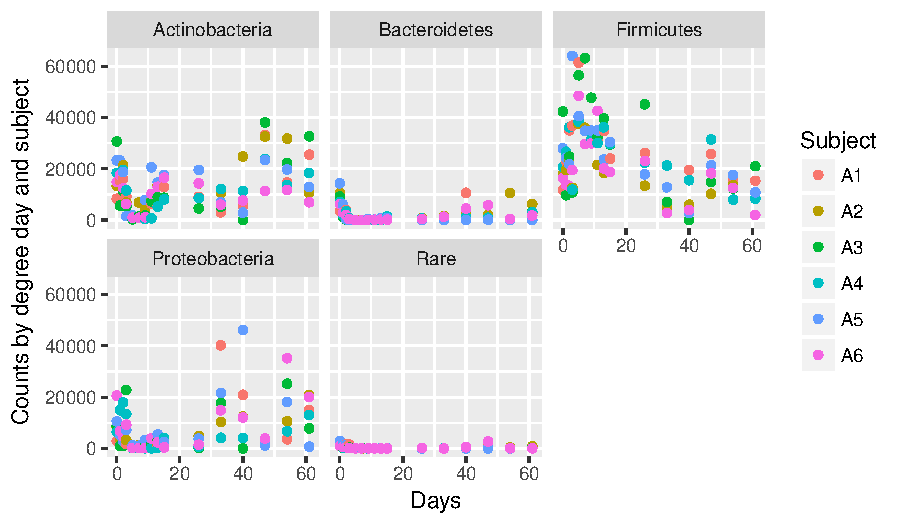
\includegraphics[width=4.5in]{phyla_scatter_counts_by_day_bacteria}
\end{figure}
\end{center}
\vspace{-0.05in}
\noindent {\scriptsize There is extensive variability in phyla counts
  between cadavers.  The same is true for families.}

\end{frame}




\begin{frame}{First 5 days: compare subjects}

\begin{center}
\begin{figure}
  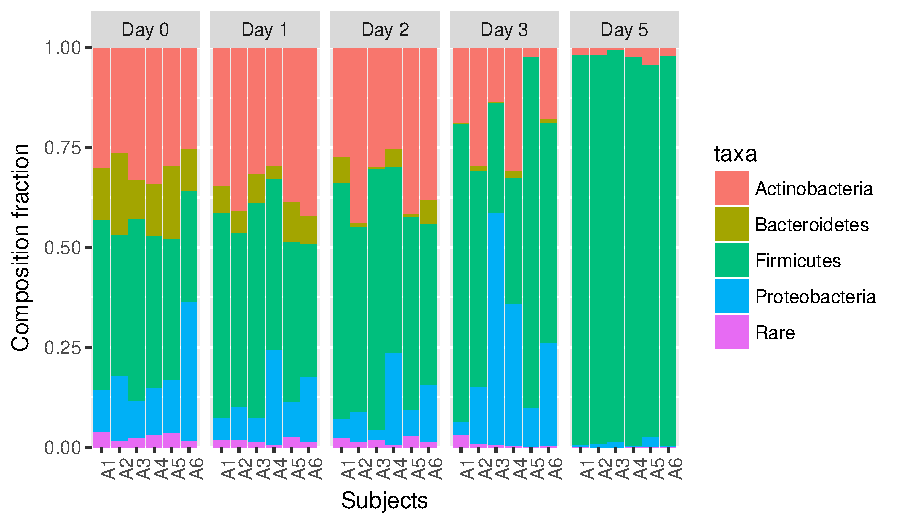
\includegraphics[width=4.5in]{phyla_first5_frac_bars_by_day_indiv}
\end{figure}
\end{center}
\vspace{-0.05in}
\noindent {\scriptsize There is some variability between cadavers, even when looking at fractions, rather than counts.  This graph shows phyla, but there is similar variability for families.}

\end{frame}




\begin{frame}{First 5 days: average fractional composition (phyla)}

\begin{center}
\begin{figure}
  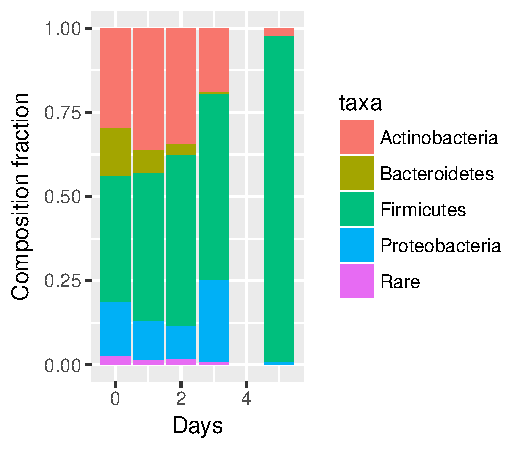
\includegraphics[width=2.5in]{phyla_first5_avgfrac_bars_by_day}
\end{figure}
\end{center}
\vspace{-0.05in}
\noindent {\scriptsize Comparing with Pechal et al (2013), Fig.~1a, our graph has less Proteobacteria and more Actinobacteria.}

\end{frame}




\begin{frame}{First 5 days: average fractional composition (families)}

\begin{center}
\begin{figure}
  \includegraphics[width=2.0in]{families_first5_avgfrac_bars_by_day}
\end{figure}
\end{center}
\vspace{-0.05in}
\noindent {\scriptsize Compare with Pechal et al (2013), Fig.~1b.  Our dataset indicates the presence of some families not present in their graph, and vice-versa.}

\end{frame}



\begin{frame}{Taxa patterns by degree days (phyla)}

\begin{center}
\begin{figure}
  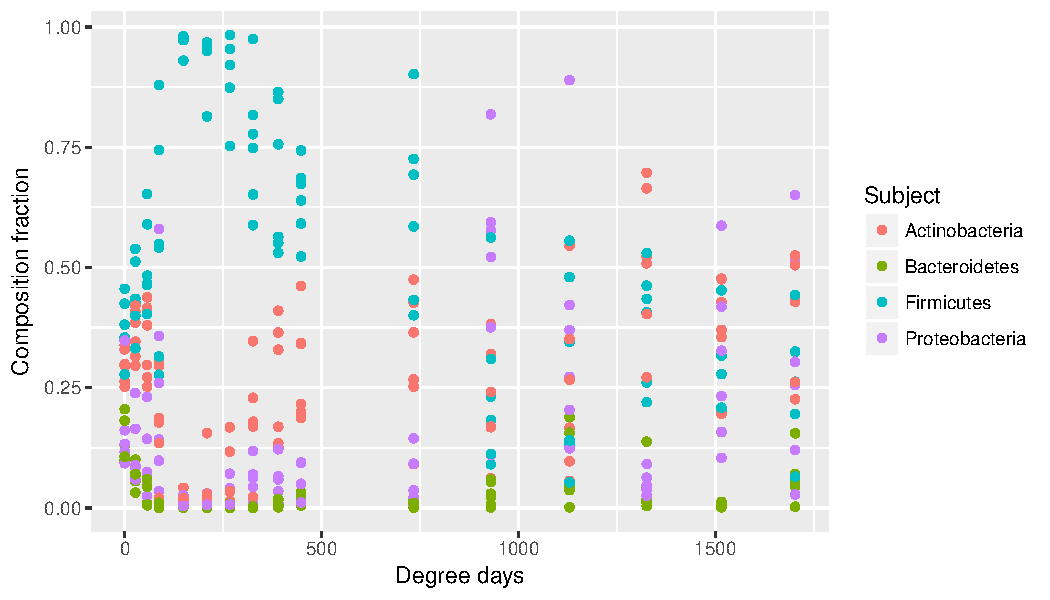
\includegraphics[width=4.5in]{phyla_scatter_frac_by_degday}
\end{figure}
\end{center}
\vspace{-0.1in}
\noindent {\scriptsize Individual cadavers are not distinguished in this graph.}

\end{frame}



\begin{frame}{Taxa patterns by degree days (families)}

\begin{center}
\begin{figure}
  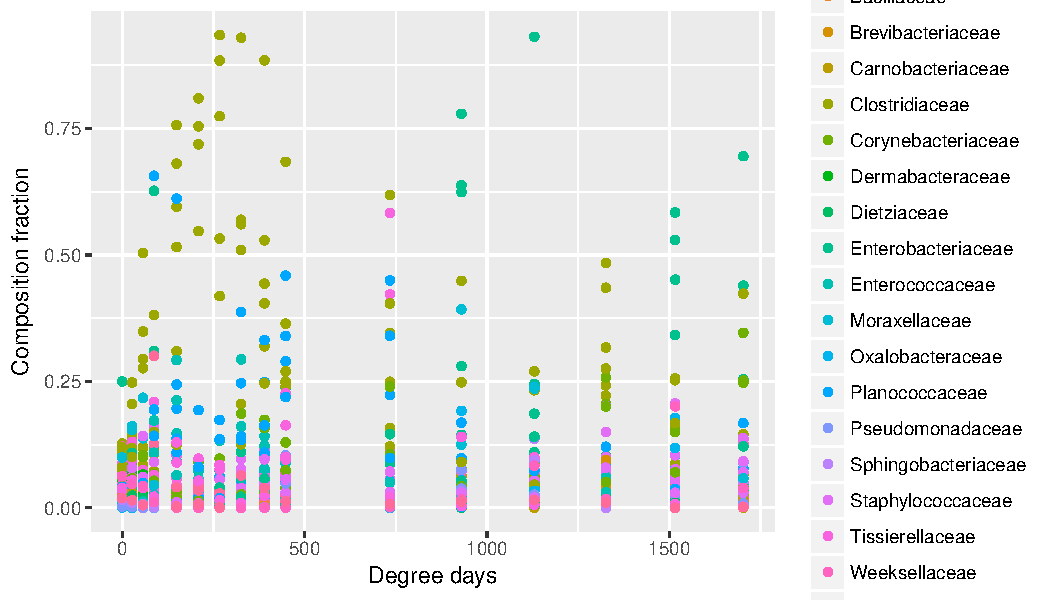
\includegraphics[width=4.5in]{families_scatter_frac_by_degday}
\end{figure}
\end{center}
\vspace{-0.1in}
\noindent {\scriptsize Individual cadavers are not distinguished in this graph.}

\end{frame}
%% %%%%%%%%%%%%%%%%%%%%%%%%%%%%%


%% %%%%%%%%%%%%%%%%%%%%%%%%%%%%%
\section{Analysis ideas}


\begin{frame}{Difficulties}
  
\begin{itemize}
\item The explanatory variables are compositional fractions (for each day and each cadaver).
\item Multicollinearity (strong dependencies among the explanatory variables) makes it difficult to use typical modeling techniques.
\item One strategy would be to use principal components analysis to summarize most of the variability with fewer (constructed) variables.
\item The predictive model will then be in terms of the principal components rather than original compositional fractions.
  \item We'll have to decide how many principal components to retain.
\end{itemize}

\end{frame}




\begin{frame}{Percentage of variability explained (phyla)}

\begin{center}
\begin{figure}
  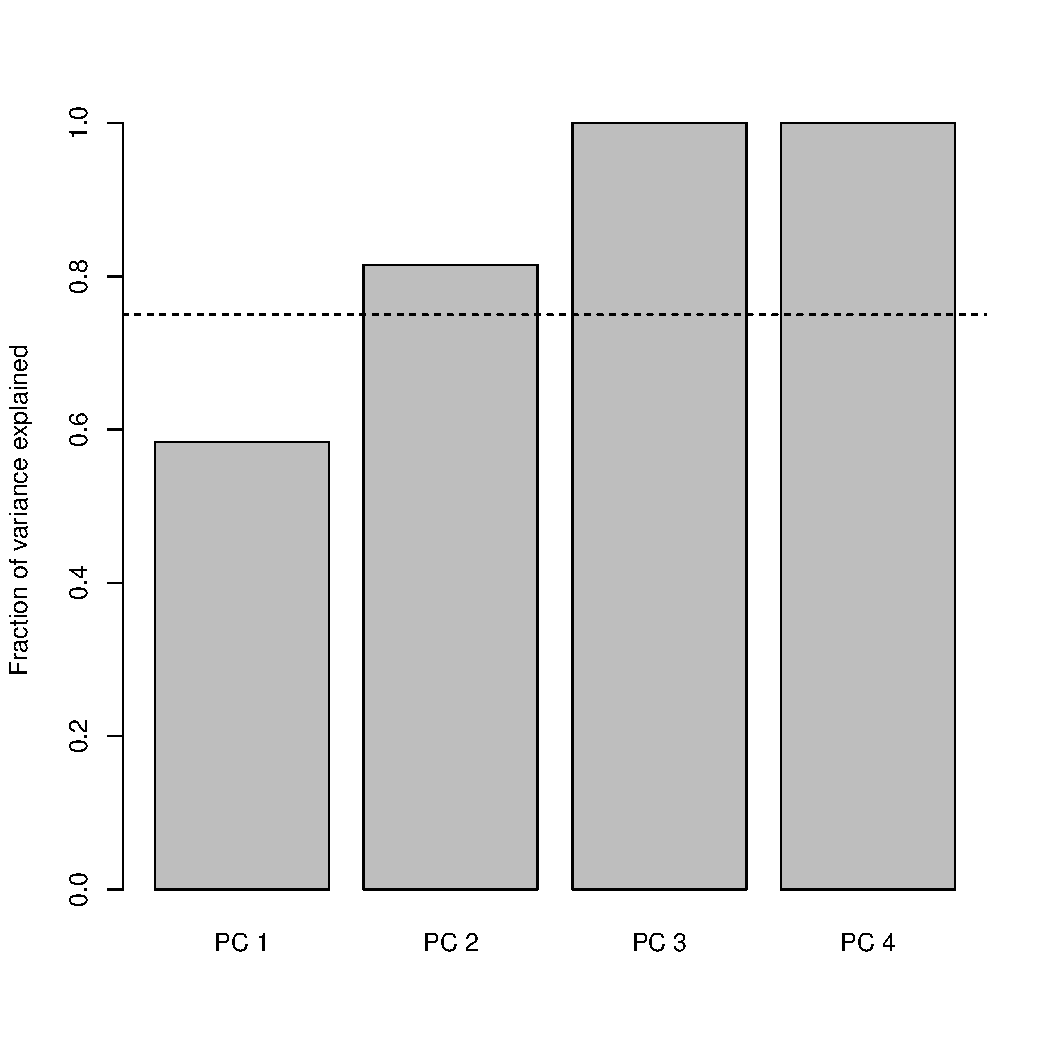
\includegraphics[width=2.5in]{phyla_prcomp_expl_barchart}
\end{figure}
\end{center}
\vspace{-0.1in}
\noindent {\scriptsize Two PCs explain more than 75\% of the variability.  Three PCs explain almost all.}

\end{frame}



\begin{frame}{Percentage of variability explained (families)}

\begin{center}
\begin{figure}
  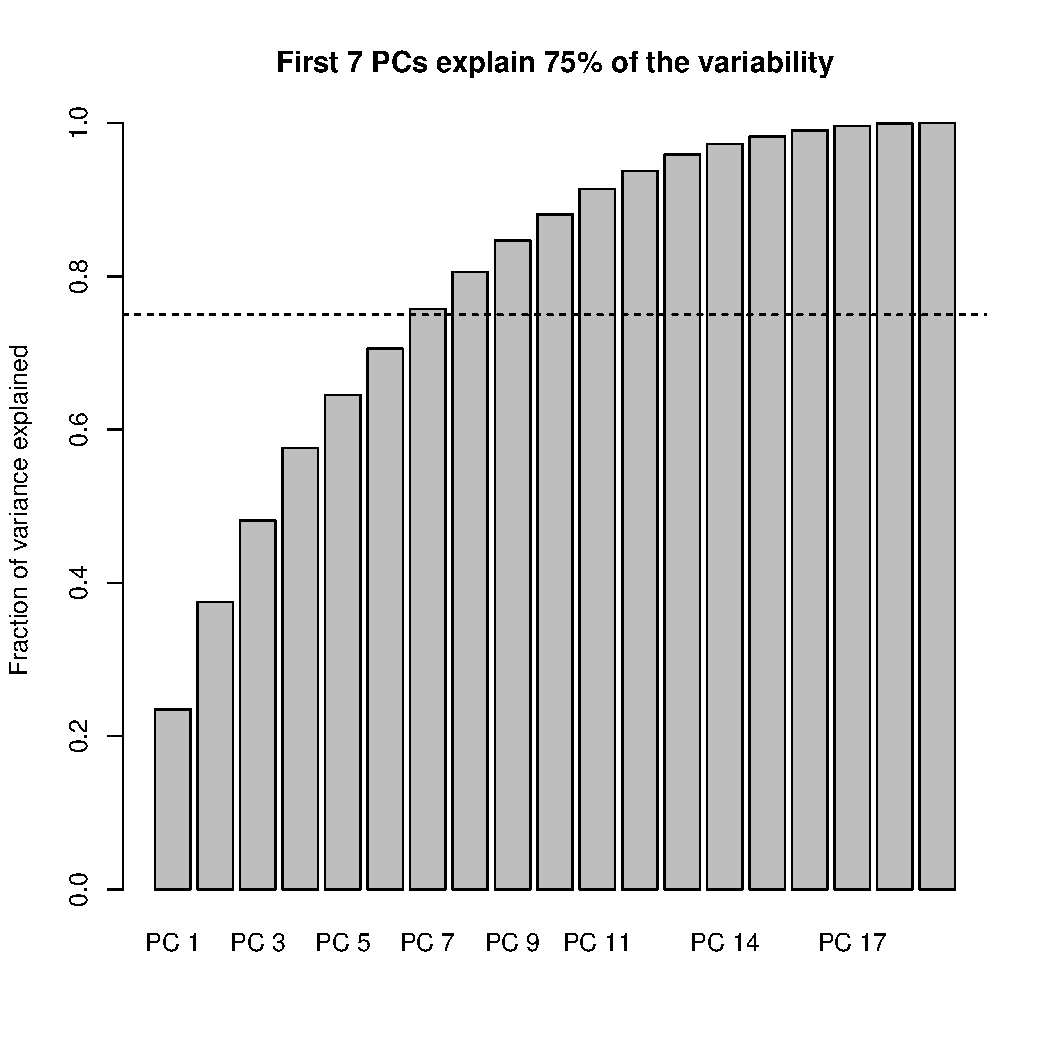
\includegraphics[width=2.5in]{families_prcomp_expl_barchart}
\end{figure}
\end{center}
\vspace{-0.1in}
\noindent {\footnotesize Seven PCs explain slightly more than 75\% of the variability.  We would have to see how sensitive any analysis is to the number of PCs retained.}

\end{frame}


\begin{frame}{Potential models}
  
  \begin{itemize}
    \item Looking at the graphs of composition fraction vs. accumulated degree days, it seems we're going to need a nonlinear model.
\item I'd like to try generalized additive models using the PCs.
\item These models allow for flexibility in the shape of the relationship.
  \item We'd want to be careful to balance flexibility with utility (avoid over-fitting, place emphasis on predictive value for some portion of dataset held in reserve).
\end{itemize}

\end{frame}



\end{document}
